\documentclass[11pt,a4paper]{article}
\usepackage[a4paper,margin=2cm]{geometry}
\usepackage[T1]{fontenc}
\usepackage{mathpazo}
\usepackage{microtype}
\usepackage{amsmath,amssymb}
\usepackage{graphicx}
\usepackage{xcolor}
\usepackage{booktabs}
\usepackage{float}
\usepackage{enumitem}
\usepackage[font=small,labelfont=bf,skip=4pt]{caption}
\usepackage[colorlinks=true,linkcolor=black,citecolor=black,urlcolor=blue!60!black]{hyperref}
\usepackage{titlesec}

\graphicspath{{figures/}}
\titleformat{\section}{\large\bfseries}{\thesection}{0.6em}{}
\titleformat{\subsection}{\normalsize\bfseries}{\thesubsection}{0.6em}{}
\titlespacing*{\section}{0pt}{8pt plus 2pt}{3pt}
\titlespacing*{\subsection}{0pt}{6pt plus 2pt}{2pt}
\setlength{\parskip}{3pt}
\setlength{\parindent}{0pt}
\setlength{\abovedisplayskip}{4pt}
\setlength{\belowdisplayskip}{4pt}
\setlength{\textfloatsep}{8pt plus 2pt}
\setlength{\intextsep}{6pt plus 2pt}
\setlist[itemize]{leftmargin=1.2em,itemsep=1pt,topsep=2pt,parsep=0pt}

\newcommand{\FHz}{F_{H0}}
\newcommand{\tentothe}[2]{$#1\times10^{#2}$}

\begin{document}

\pagenumbering{gobble}
\begin{titlepage}
\centering
\vspace*{4cm}
{\LARGE\bfseries When Does a Moored Tanker Fishtail?\par}
\vspace{0.6cm}
{\Large Pitchfork and Hopf Bifurcations of a Single-Point-Moored\\[2pt] Tanker in Steady Current\par}
\vspace{2.5cm}
{\large Course Project Report\par}
\vspace{2.5cm}
{\large Aarav Patel (NA23B014)\par}
\vspace{0.25cm}
{\large Kaeshav Siddarthan R M (NA23B049)\par}
\vfill
{\large OE5320 Non Linear Problems in Ocean Engineering\par}
\vspace{0.3cm}
{\large November 2026\par}
\vspace*{2cm}
\end{titlepage}

\tableofcontents
\clearpage
\pagenumbering{arabic}

\section{Introduction}
A single-point mooring holds a tanker at the bow by one hawser running to a buoy and leaves it free to weathervane. The
ship does not always settle behind the buoy. Under some conditions it swings from side to side and keeps swinging even
in a perfectly steady current. This motion is called fishtailing, and it matters because the hawser tension rises and
falls with every swing.

If the bow moves off the current, the Munk moment tries to turn the hull further broadside, while the hawser tension and
the side force on the hull pull it back. Depending on where the hawser is tied, how long it is and how large the
friction drag is, the ship trails straight, rests at a steady angle or fishtails. Simos \cite{simos} built a
hydrodynamic model for this problem and tested it on a 1:90 tanker model, and fishtailing has also been seen in flume
tests \cite{aghamohammadi}. Because the current is steady, the swing is a self-excited limit cycle, so the problem is a
natural fit for the bifurcation theory of our course text \cite{strogatz}. We rebuilt Simos's model and studied six
cases: the attachment point, friction, hawser length, a side wind, a hold-back tug and a stern thruster.

\section{Methodology}
\textbf{Ship.} We use the Vidal de Negreiros, a 320~m VLCC, in the fully loaded condition. Its particulars, taken from
Simos \cite{simos}, are listed in Table~\ref{tab:ship}.

\begin{table}[H]
\centering\footnotesize
\caption{Particulars of the Vidal de Negreiros (full scale, fully loaded).}
\label{tab:ship}
\begin{tabular}{@{}lc@{\hspace{2.5em}}lc@{}}
\toprule
Length $L$ (m) & 320 & Mass $M$ (kg) & \tentothe{3.219}{8}\\
Beam $B$ (m) & 54.5 & Yaw inertia $I_z$ (kg\,m$^2$) & \tentothe{2.06}{12}\\
Draft $T$ (m) & 21.47 & Added mass, surge $M_{11}$ (kg) & \tentothe{1.848}{7}\\
Block coefficient $C_B$ & 0.83 & Added mass, sway $M_{22}$ (kg) & \tentothe{2.725}{8}\\
CG forward of midship $x_{CG}$ (m) & 9.81 & Added yaw inertia $M_{66}$ (kg\,m$^2$) & \tentothe{1.579}{12}\\
Cross-flow drag coefficient $C_Y$ & 0.84 & Sway--yaw coupling $M_{26}$ (kg\,m) & \tentothe{2.209}{9}\\
\bottomrule
\end{tabular}
\end{table}

\textbf{Model.} The hawser is a rigid link of length $L_H$, tied a distance $x_A$ forward of midship
(Fig.~\ref{fig:schematic}). With the buoy at the origin and the $X$ axis pointing upstream, the attachment point and
midship are at
\begin{equation}
\mathbf A=L_H(-\cos\gamma,\ \sin\gamma),\qquad \mathbf O=\mathbf A-x_A(\cos\psi,\ \sin\psi),
\end{equation}
so the hawser angle $\gamma$ and the heading $\psi$ fix the position of the ship, and the state is
$(\gamma,\psi,\dot\gamma,\dot\psi)$. Differentiating $\mathbf O$ and adding the current $U$ gives the velocities
relative to the water,
\begin{equation}
u = U\cos\psi + L_H\dot\gamma\sin(\gamma+\psi),\qquad
v = -U\sin\psi + L_H\dot\gamma\cos(\gamma+\psi) - x_A\dot\psi,\qquad
r=\dot\psi.
\end{equation}
The hawser pulls the attachment point towards the buoy with force $F_H$, which gives
$F_X=F_H\cos(\gamma+\psi)$, $F_Y=-F_H\sin(\gamma+\psi)$ and a yaw moment $-x_AF_H\sin(\gamma+\psi)$. With the water
loads $X_R$, $Y_R$, $N_R$ from Simos's model, $m_{26}=Mx_{CG}+M_{26}$ and $I_{66}=I_Z+M_{66}$ (yaw inertia about
midship), the manoeuvring equations in surge, sway and yaw are
\begin{equation}
\begin{aligned}
(M+M_{11})\dot u-(M+M_{22})vr-m_{26}r^2&=X_R+F_H\cos(\gamma+\psi),\\
(M+M_{22})\dot v+(M+M_{11})ur+m_{26}\dot r&=Y_R-F_H\sin(\gamma+\psi),\\
I_{66}\dot r+m_{26}(\dot v+ur)&=N_R-x_AF_H\sin(\gamma+\psi).
\end{aligned}
\end{equation}
Since the hawser length is fixed, $F_H$ is an unknown. Writing $\dot u=L_H s\,\ddot\gamma+a_u$ and
$\dot v=L_H c\,\ddot\gamma-x_A\ddot\psi+a_v$, with $s=\sin(\gamma+\psi)$, $c=\cos(\gamma+\psi)$ and $a_u$, $a_v$ the
known remainders, turns the three equations into a linear system that we solve at every time step:
{\small
\begin{equation}
\begin{bmatrix}
(M+M_{11})L_Hs & 0 & -c\\
(M+M_{22})L_Hc & m_{26}-(M+M_{22})x_A & s\\
m_{26}L_Hc & I_{66}-m_{26}x_A & x_As
\end{bmatrix}
\begin{bmatrix}\ddot\gamma\\\ddot\psi\\F_H\end{bmatrix}
=
\begin{bmatrix}
X_R+(M+M_{22})vr+m_{26}r^2-(M+M_{11})a_u\\
Y_R-(M+M_{11})ur-(M+M_{22})a_v\\
N_R-m_{26}(a_v+ur)
\end{bmatrix}.
\end{equation}}

\begin{figure}[t]
\centering
\begin{minipage}[b]{0.47\linewidth}\centering
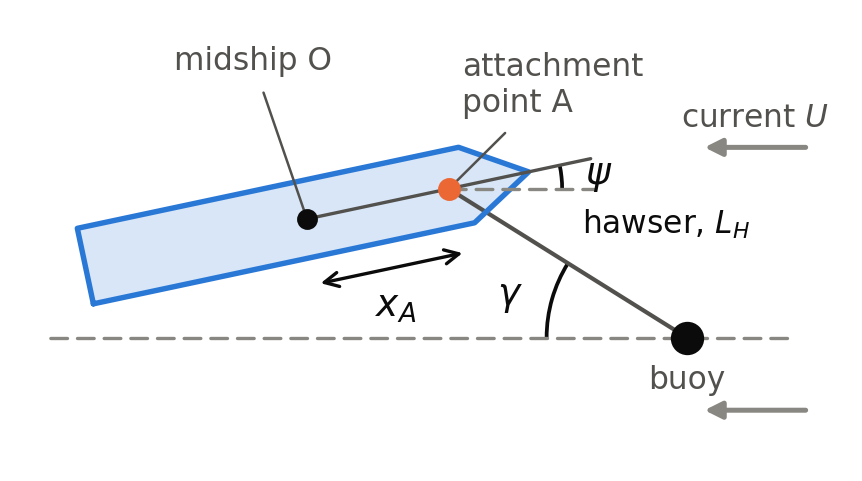
\includegraphics[width=\linewidth]{fig01_schematic}
\caption{Plan view of the mooring. $\gamma$ and $\psi$ are positive to port; the bow is at $x_A/L=0.5$.}
\label{fig:schematic}
\end{minipage}\hfill
\begin{minipage}[b]{0.5\linewidth}\centering
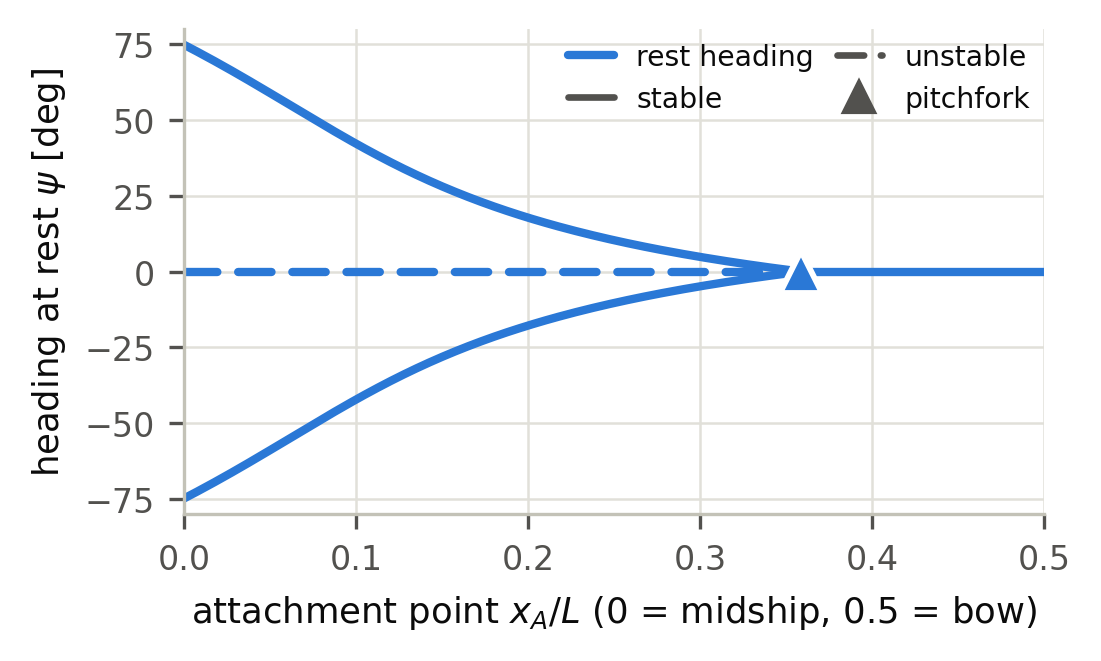
\includegraphics[width=\linewidth]{fig02_pitchfork}
\caption{Rest heading against $x_A/L$ ($L_H/L=0.5$, $C_F=0.05$).}
\label{fig:pitchfork}
\end{minipage}
\end{figure}

\textbf{Current speed.} Time is measured as $t^*=Ut/L$, the time the current takes to pass one ship length. In these
units the current speed survives only through the skin-friction coefficient $C_F$, which falls as the current speeds
up, so we use $C_F$ as the speed parameter. It is about 0.02--0.05 for
the 1:90 tank model and about 0.010 for the real ship in a 1~m/s current. When the ship trails straight, the hawser
tension equals the friction drag, $\FHz=C_F\tfrac12\rho U^2LT$, and all tug, wind and thruster forces are given as
multiples of $\FHz$.

\textbf{Stability and limit cycles.} A rest position is stable when all four eigenvalues $\lambda=\sigma\pm i\omega$ of
the linearised system have negative real parts. A real eigenvalue crossing zero signals a pitchfork or a fold, and a
complex pair crossing the imaginary axis signals a Hopf bifurcation. Limit cycles were found by simulation and, near a Hopf point, by a
shooting method, with Floquet multipliers for their stability. Our Hopf boundary agrees with Simos's published curve to within $+0.5$\,\% on average
(Fig.~\ref{fig:hawser}a).

\textbf{Initial conditions.} Each run starts from straight trailing with a small nudge, $\gamma=3^\circ$,
$\psi=1^\circ$ and zero rates. In parameter sweeps each run starts from where the previous one ended, and sweeping in
both directions reveals any hysteresis. In the control
studies the runs start from the fully developed fishtail, with the control switched on at $t^*=0$, and in the wind
study they start with the ship resting at an angle to port.


\section{Results}\label{sec:results}

\subsection{Attachment point: pitchfork}
\begin{itemize}
\item \textbf{Set-up:} $x_A/L$ varied (0 = midship, 0.5 = bow); $L_H/L=0.5$ and a high friction $C_F=0.05$ held
fixed, so the ship never fishtails here.
\item At rest the hawser force drops out of the equations, leaving
\[
N_R(\psi)-x_A\,Y_R(\psi)=0,
\]
so the rest heading depends only on $x_A/L$: the water's turning moment about the hawser point must vanish.
\item Forward of $x_A/L=0.359$ the hull's side force acts like a weathervane tail and the ship trails straight. Aft of
it the Munk moment wins and the ship settles at a steady angle to port or starboard, e.g.\ $\psi=10.3^\circ$ at
$x_A/L=0.25$: a pitchfork (Fig.~\ref{fig:pitchfork}).
\item A real eigenvalue (a slow sideways drift) crosses zero. Just past the pitchfork, straight trailing has $+0.034$ and
the angled positions $-0.034$, an exchange of stability.
\item It is supercritical: the new branches are stable and grow from zero. They grow linearly (log--log slope 1.00), not
as a square root, because cross-flow drag varies as $\psi|\psi|$, giving $\dot\psi=r\psi-q\psi|\psi|$ in place of
Strogatz's $\dot x=rx-x^3$.
\end{itemize}

\subsection{Friction: Hopf bifurcation}
\begin{figure}[t]
\centering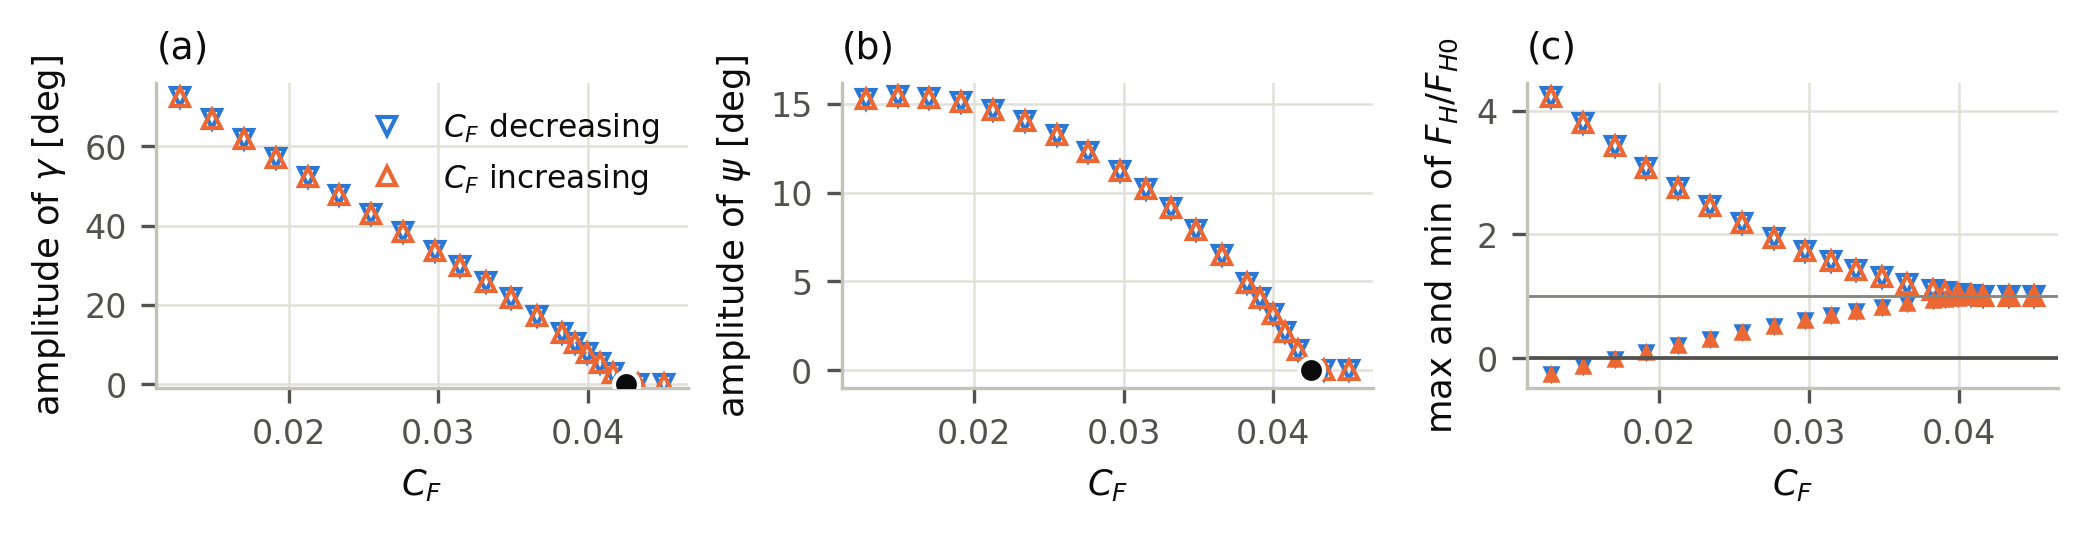
\includegraphics[width=\linewidth]{fig03_friction}
\caption{Effect of friction ($x_A/L=L_H/L=0.5$): swing amplitude of (a) $\gamma$ and (b) $\psi$, and (c) the largest (open)
and smallest (filled) hawser force. $\bullet$ marks the Hopf point.}
\label{fig:friction}
\end{figure}
\begin{itemize}
\item \textbf{Set-up:} $C_F$ varied (lower = faster current); hawser at the bow ($x_A/L=0.5$) and $L_H/L=0.5$.
\item The ship on its hawser behaves like a pendulum whose restoring force is the tension $\FHz$, which is proportional
to $C_F$.
\item A complex pair $\lambda=\sigma\pm i\omega$ crosses the imaginary axis ($\sigma=0$, $\omega\ne0$) at
$C_F=0.0425$, with $\omega=0.738\,U/L$, a period of $8.5\,L/U$. This is a Hopf bifurcation.
\item Below it the swing grows and levels off at a fixed size: $\gamma=\pm33^\circ$, $\psi=\pm11^\circ$ at $C_F=0.03$,
and $\gamma=\pm72^\circ$ at $C_F=0.013$ (Fig.~\ref{fig:friction}).
\item Sweeps down and up give the same curve, so there is no hysteresis and the Hopf bifurcation is supercritical.
Floquet multipliers confirm that the cycles are stable.
\item The amplitude $a$ grows in proportion to the distance past the Hopf point (slope 0.98), since averaging with
quadratic drag gives $\dot a=\mu a-ca^2$ and hence $a^*=\mu/c$.
\item Below $C_F\approx0.017$ the hawser tension would turn negative for part of each swing, which a real rope cannot do.
\end{itemize}

\subsection{Hawser length: Hopf bifurcation}
\begin{figure}[t]
\centering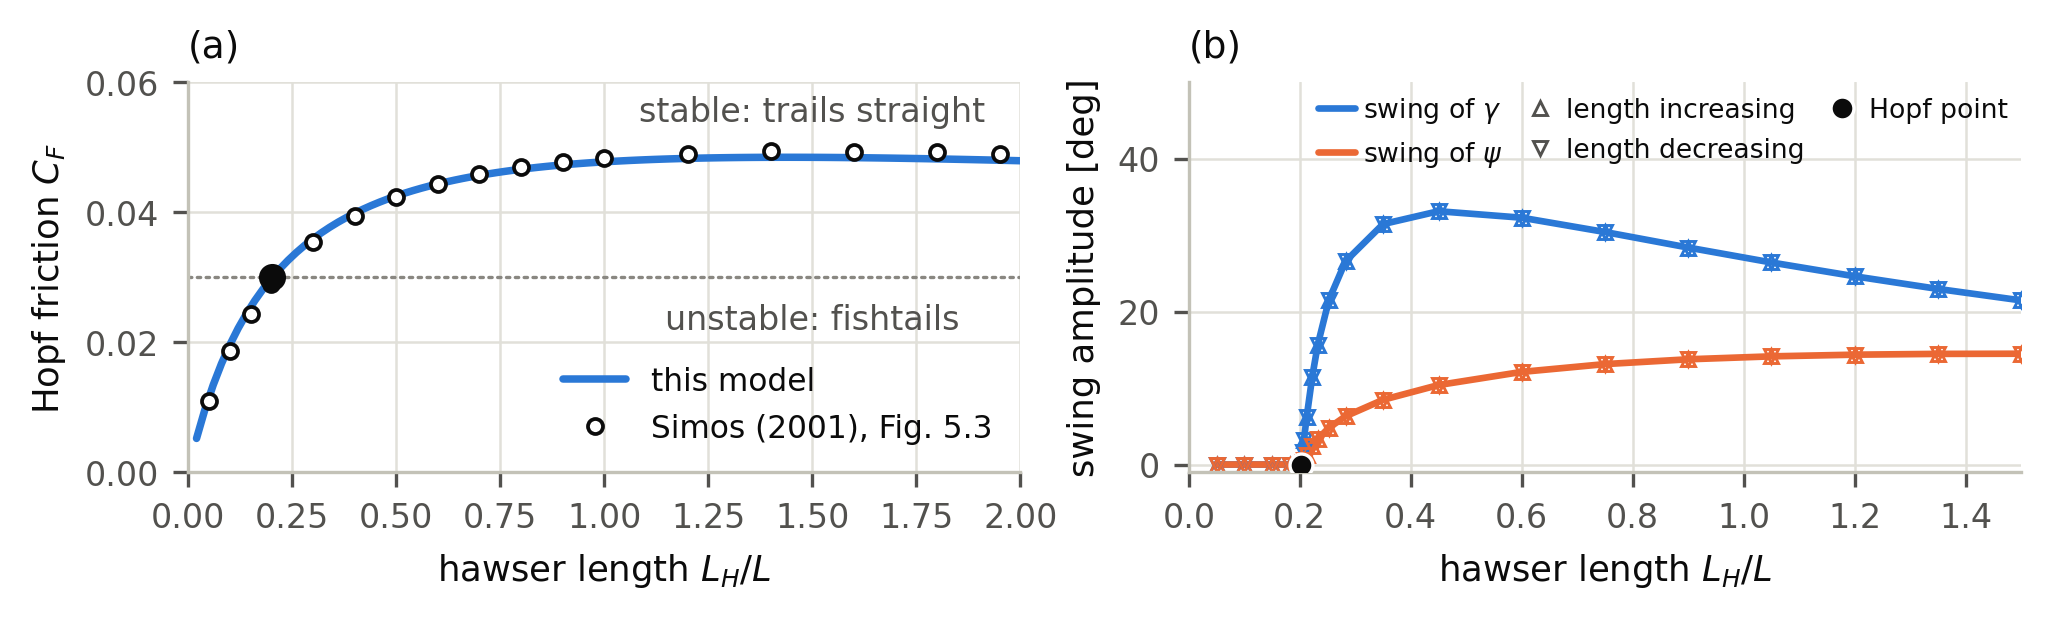
\includegraphics[width=\linewidth]{fig04_hawser_length}
\caption{Effect of hawser length. (a) Hopf boundary of straight trailing, compared with Simos \cite{simos}; the dotted
line marks $C_F=0.03$. (b) Swing amplitude at $C_F=0.03$ for increasing and decreasing hawser length.}
\label{fig:hawser}
\end{figure}
\begin{itemize}
\item \textbf{Set-up:} $L_H/L$ varied; hawser at the bow and $C_F=0.03$.
\item A short hawser is a stiff, well-damped pendulum. The Hopf condition $\sigma(L_H)=0$ is met at $L_H/L=0.202$, a
hawser of about 65~m, and any longer hawser fishtails.
\item Over all lengths (Fig.~\ref{fig:hawser}a) the boundary rises from $C_F=0.0298$ at $L_H/L=0.2$ to $0.0478$ at
$1.0$, so shorter hawsers are safer. The real ship, at $C_F\approx0.010$, fishtails for all but the shortest hawsers.
\item Sweeps of increasing and decreasing length give the same swing, to within $0.05^\circ$. It grows from zero at the
Hopf point and every cycle is stable, so this Hopf bifurcation is also supercritical (Fig.~\ref{fig:hawser}b).
\item The swing angle $\gamma$ peaks at about $\pm33^\circ$ near $L_H/L=0.5$ and then falls slowly, but the bow's
sideways sweep keeps growing, from $\pm87$~m at $L_H/L=0.5$ to $\pm176$~m at $1.5$, while the heading swing levels off
near $\pm14.5^\circ$.
\end{itemize}

\subsection{Wind: imperfect pitchfork}
\begin{figure}[t]
\centering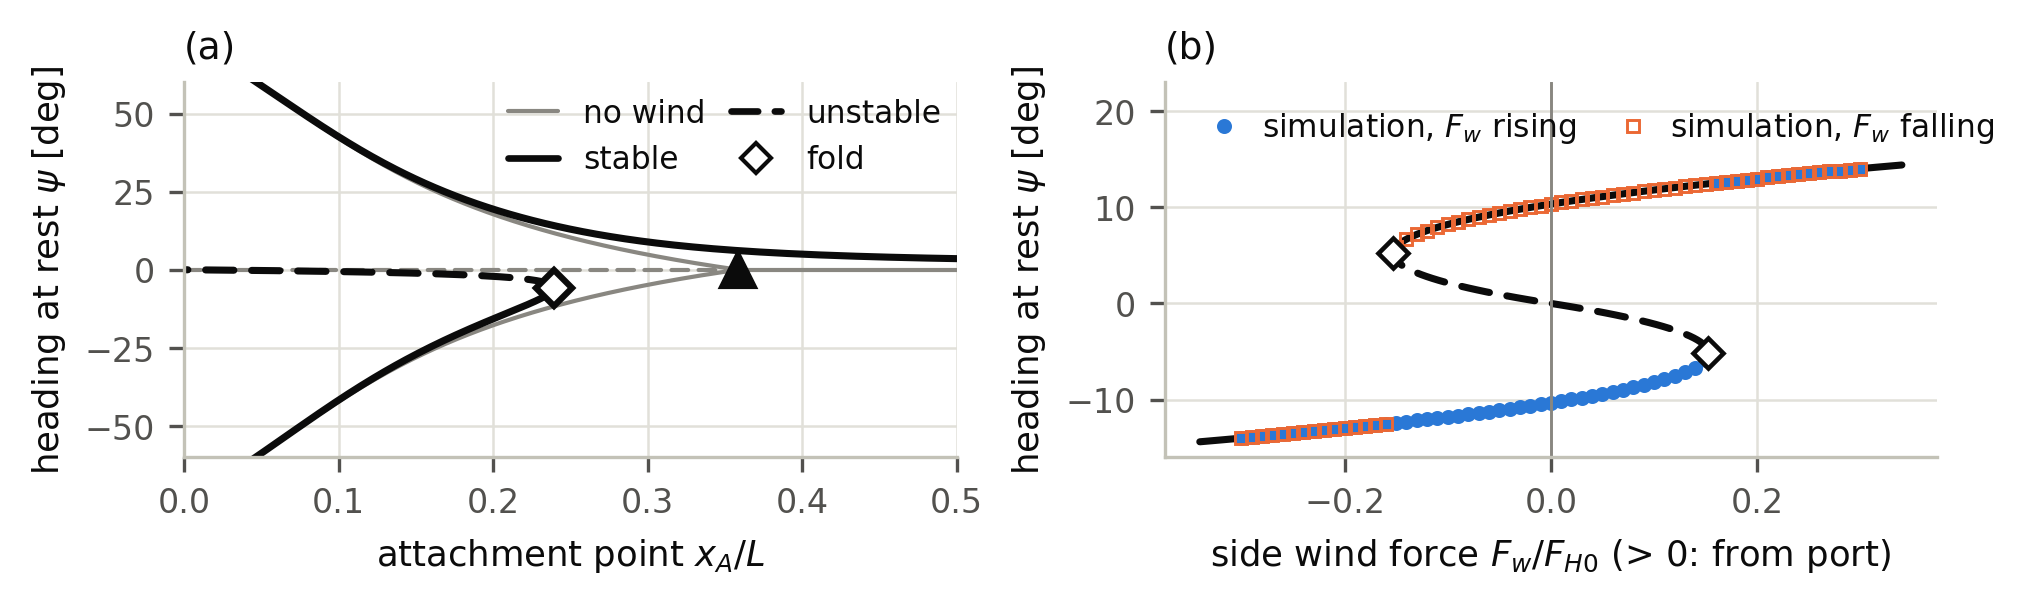
\includegraphics[width=0.93\linewidth]{fig05_wind}
\caption{Effect of a side wind. (a) Imperfect pitchfork for a beam wind of $0.20\,\FHz$ from port, over the no-wind diagram. (b)
Hysteresis at $x_A/L=0.25$; simulated sweeps follow the stable branches and jump just past the folds.}
\label{fig:wind}
\end{figure}
\begin{itemize}
\item \textbf{Set-up:} wind force $F_w/\FHz$ and direction varied; $x_A/L=0.25$ (aft of the pitchfork), $L_H/L=0.5$
and $C_F=0.05$. The wind is a constant force acting at midship.
\item A side wind breaks the mirror symmetry. The pitchfork splits into one smooth branch and one that ends at a fold
(Fig.~\ref{fig:wind}a). The reduced equation is Strogatz's imperfect pitchfork with $\psi|\psi|$ in place of $x^3$,
\[
\dot\psi=h+r\psi-q\psi|\psi|,\qquad \text{folds at } h=\pm\frac{r^2}{4q},
\]
where $h$ is the side part of the wind force.
\item The ship keeps its side until the wind passes the fold, at $\pm0.153\,\FHz$ for a beam wind, and then swings
across. It does not swing back when the wind drops: hysteresis (Fig.~\ref{fig:wind}b).
\item At the fold a stable and an unstable rest position meet with a zero eigenvalue and vanish (saddle-node). Other
directions need more wind, and wind from ahead or astern keeps the pitchfork perfect.
\item The ship ends up on the upwind side. The wind acts aft of the hawser point and turns the bow into the wind, and the
hull's lift in the current then carries the ship that way.
\end{itemize}

\subsection{Control by tug}
\begin{figure}[t]
\centering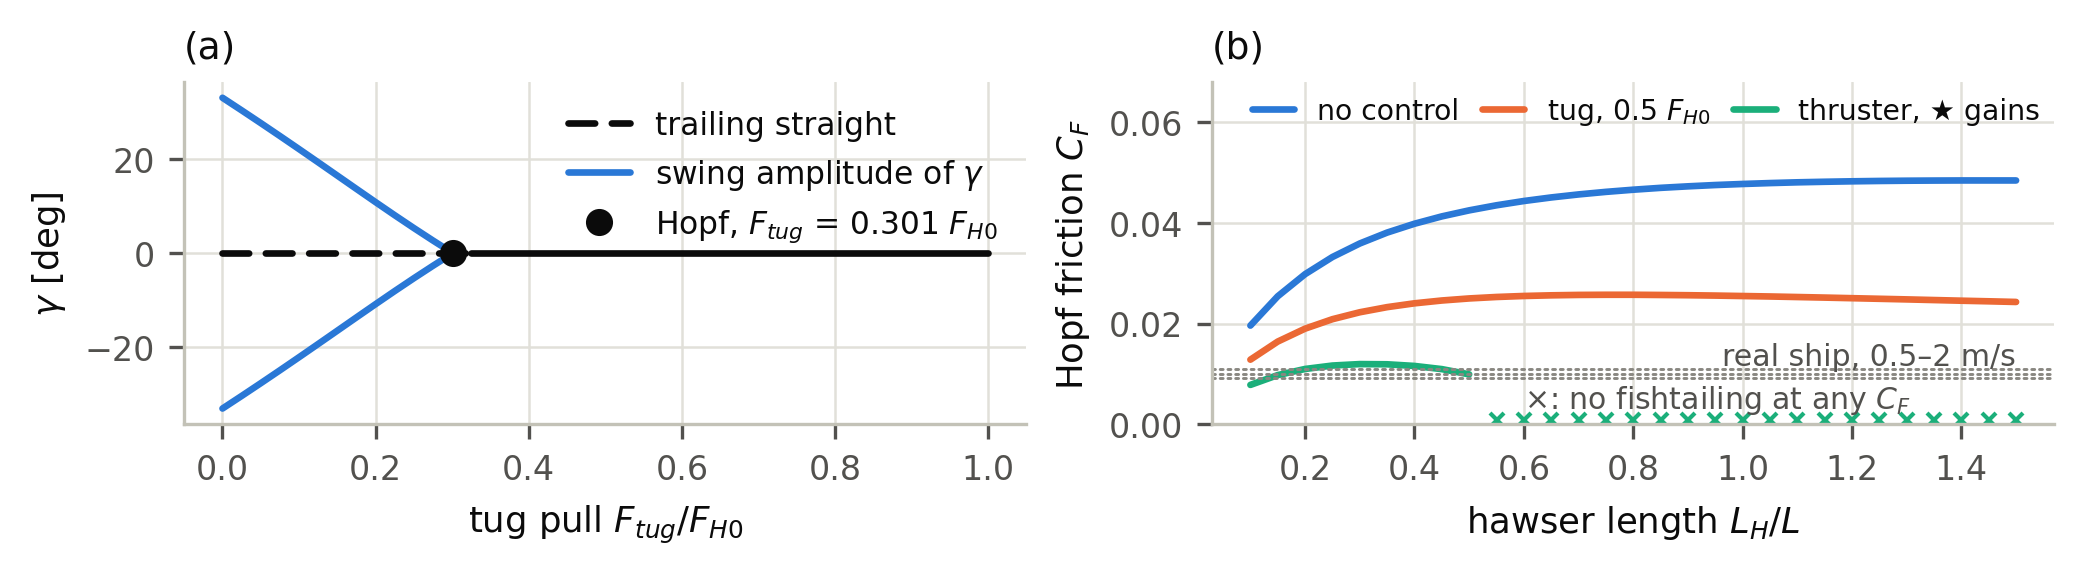
\includegraphics[width=0.93\linewidth]{fig06_tug}
\caption{(a) Hold-back tug at $C_F=0.03$: the swing shrinks to a Hopf point. (b) Hopf boundary with and without control at
$x_A/L=0.5$; the thruster uses the gains $\bigstar$ of Fig.~\ref{fig:thruster}.}
\label{fig:tug}
\end{figure}
\begin{itemize}
\item \textbf{Set-up:} tug pull $F_{tug}/\FHz$ and $C_F$ varied; hawser at the bow and $L_H/L=0.5$.
\item A hold-back tug at the stern pulls steadily downstream. It raises the hawser tension to $\FHz+F_{tug}$, and once
the bow swings off, the sideways part of its pull, about $F_{tug}\psi$, acts like a weathervane tail.
\item At $C_F=0.03$ the swing shrinks linearly with the pull and disappears at a Hopf point, $F_{tug}=0.301\,\FHz$
(Fig.~\ref{fig:tug}a).
\item A faster current needs much more pull: $0.66\,\FHz$ at $C_F=0.022$ and $2.24\,\FHz$ at $C_F=0.010$, the real ship
at about 1~m/s.
\item A pull of $0.5\,\FHz$ lowers the Hopf friction at $L_H/L=0.5$ from $0.0425$ to $0.025$ (Fig.~\ref{fig:tug}b).
\end{itemize}

\subsection{Control by stern thruster}
\begin{figure}[t]
\centering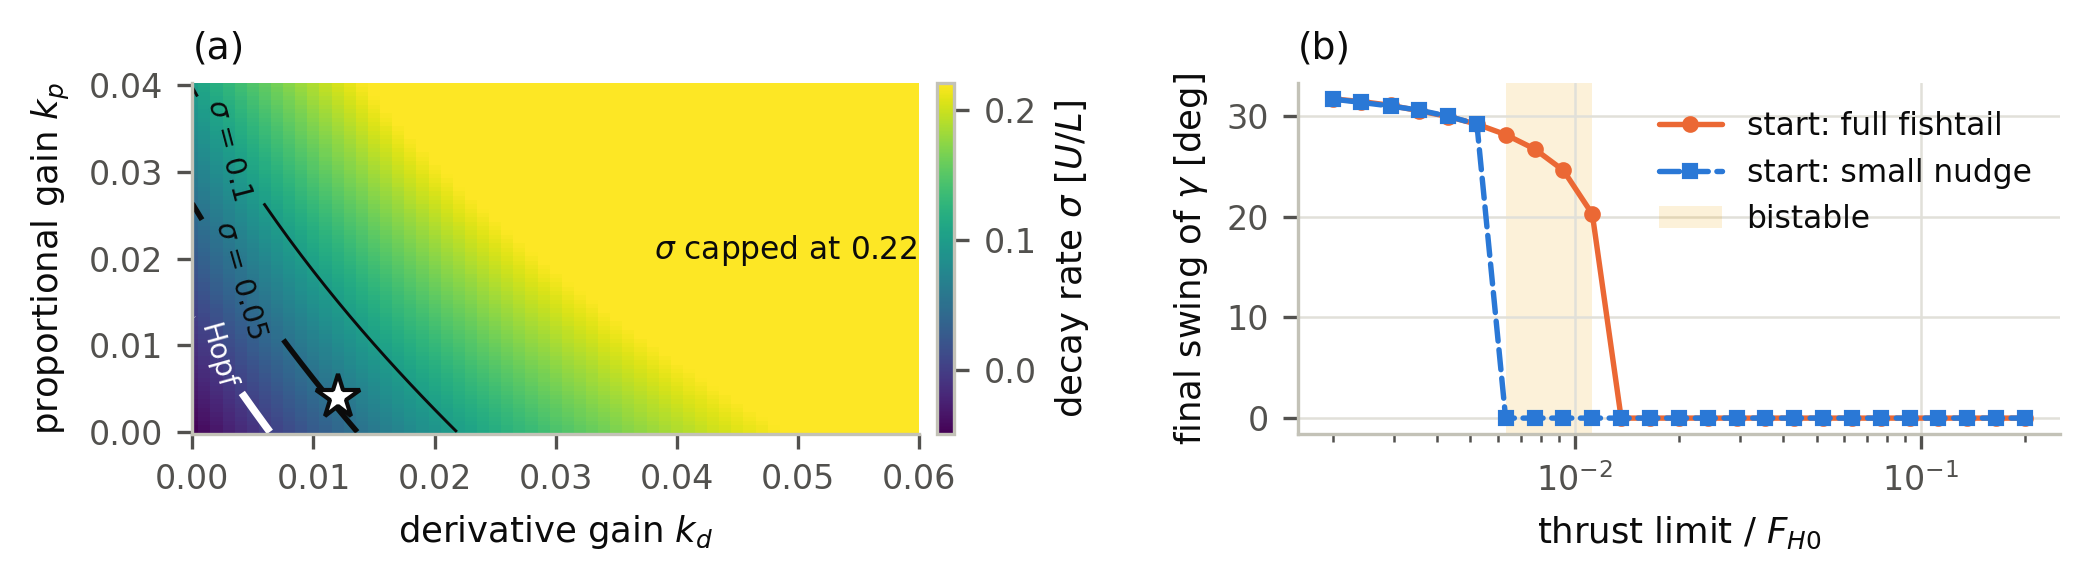
\includegraphics[width=0.86\linewidth]{fig07_thruster}
\caption{Stern thruster at $C_F=0.03$. (a) Decay rate over the gain plane; $\bigstar$ marks the least-thrust gains. (b)
Swing left after $600\,t^*$ against the thrust limit; the shaded band is bistable.}
\label{fig:thruster}
\end{figure}
\begin{itemize}
\item \textbf{Set-up:} gains $k_d$, $k_p$ and thrust limit varied; $x_A/L=L_H/L=0.5$ and $C_F=0.03$.
\item The ship's own stern thruster, at $x_T=-L/2$, follows a PD law on the heading:
\[
N_c^*=-k_p\psi-k_dr^*,\qquad Y_T=\frac{N_c}{x_T},\qquad |Y_T|\le\text{limit}\times\FHz,
\]
where $N_c^*=N_c/(\tfrac12\rho U^2L^2T)$ and $r^*=rL/U$.
\item $k_d$ adds the damping that the Hopf instability lacks: $k_d=0.0064$ alone stops the swing, or $k_p=0.0131$ alone.
\item The gains needing the least thrust for a decay rate $\sigma=-\max\operatorname{Re}\lambda\ge0.05\,U/L$ are
$k_p=0.004$, $k_d=0.012$, with a peak thrust of $0.082\,\FHz$ (Fig.~\ref{fig:thruster}a).
\item One eigenvalue, $-0.221\,U/L$, a slow sideways drift that heading control cannot see, never moves, so
$\sigma\le0.22$.
\item A thrust limit does not change the eigenvalues but matters for large swings. Between $0.0063$ and
$0.0113\,\FHz$ the system is bistable: the full fishtail survives while a small nudge dies out
(Fig.~\ref{fig:thruster}b).
\item With these gains the Hopf friction drops to $0.0099$ at $L_H/L=0.5$, and for $L_H/L\ge0.55$ fishtailing is gone at
every $C_F$ (Fig.~\ref{fig:tug}b).
\end{itemize}

\section{Conclusions and limitations}
Each behaviour of the moored ship matches a standard bifurcation (Table~\ref{tab:summary}), and because the limiting
force is quadratic drag the branches grow linearly.
\begin{table}[H]
\centering\footnotesize
\caption{Bifurcations found in the six cases.}
\label{tab:summary}
\begin{tabular}{@{}llll@{}}
\toprule
Case & Parameter & Bifurcation & Threshold\\
\midrule
Attachment point & $x_A/L$ & Supercritical pitchfork & 0.359\\
Friction & $C_F$ & Supercritical Hopf & 0.0425\\
Hawser length & $L_H/L$ & Supercritical Hopf & 0.202 ($C_F=0.03$)\\
Wind & $F_w/\FHz$ & Imperfect pitchfork, hysteresis & folds at $\pm0.153$ (beam wind)\\
Tug & $F_{tug}/\FHz$ & Hopf & 0.301 ($C_F=0.03$)\\
Thruster & $k_d$, $k_p$ & Hopf, bistable with a thrust limit & $k_d=0.0064$ or $k_p=0.0131$\\
\bottomrule
\end{tabular}
\end{table}
\begin{itemize}
\item The hawser is rigid. In a separate run with a measured nylon rope law \cite{huang} the boundaries moved by less
than 5\,\%, but at 1~m/s the rope was slack 74\,\% of the time and snatch loads reached $14\,\FHz$.
\item Flume tests have shown a subcritical Hopf bifurcation \cite{aghamohammadi}, unlike our model, so the type may
depend on the set-up.
\item The wind is a constant force, tug and thruster sizes are ratios as we found no cited VLCC values, and the tug
as a cure for fishtailing is a result of our model only.
\item An interactive version of these results is available at\\
\url{https://aaravpatel007.github.io/Moored-Tanker-Fishtailing/interactive/}.
\end{itemize}

\begingroup
\footnotesize
\begin{thebibliography}{9}
\addcontentsline{toc}{section}{References}
\setlength{\itemsep}{0pt}\setlength{\parskip}{0pt}
\bibitem{simos} A.\,N. Simos, \emph{Modelo hidrodin\^amico heur\'istico para an\'alise de navios petroleiros amarrados
sujeitos \`a a\c{c}\~ao de correnteza}, PhD thesis, Escola Polit\'ecnica, Univ. S\~ao Paulo, 2001.
\bibitem{strogatz} S.\,H. Strogatz, \emph{Nonlinear Dynamics and Chaos}, 2nd ed., Westview Press.
\bibitem{aghamohammadi} F. Aghamohammadi, J.\,M.\,T. Thompson, An experimental study of the large amplitude
fish-tailing instabilities of a tanker at a single point mooring, \emph{Appl. Ocean Res.} 12(1), 25--33, 1990.
\bibitem{huang} H. Huang et al., Investigation into fishtailing effect of oil tankers moored at pile-founded column
SPM systems, \emph{J. Mar. Sci. Eng.} 14, 770, 2026.
\end{thebibliography}
\endgroup

\end{document}
